\documentclass[border=4pt]{standalone}
\usepackage{tikz}
\usetikzlibrary{arrows.meta,positioning,shapes.misc}

\begin{document}
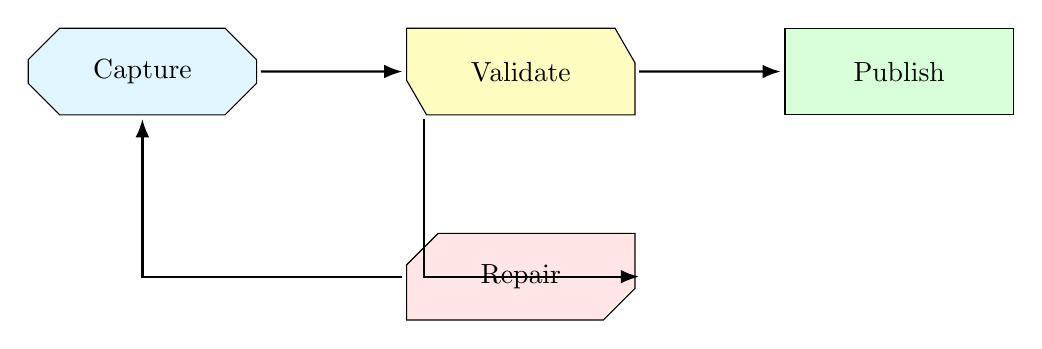
\begin{tikzpicture}[
  >=Latex,
  node distance=14mm and 18mm,
  stage/.style={shape=chamfered rectangle,draw,fill=cyan!12,
    chamfered rectangle angle=45,chamfered rectangle sep=2mm,
    minimum width=29mm,minimum height=11mm,outer sep=1.5pt},
  flow/.style={->,thick}
]
  \node[stage] (capture) {Capture};
  \node[stage,right=of capture,chamfered rectangle angle=30,
    chamfered rectangle corners={north east,south west},fill=yellow!25] (validate) {Validate};
  \node[stage,right=of validate,chamfered rectangle corners=chamfer none,
    fill=green!15] (publish) {Publish};
  \node[stage,below=of validate,chamfered rectangle corners={north west,south east},
    fill=red!10] (repair) {Repair};

  \draw[flow] (capture) -- (validate);
  \draw[flow] (validate) -- (publish);
  \draw[flow] (validate.after south west) |- (repair.east);
  \draw[flow] (repair.west) -| (capture.south);
\end{tikzpicture}
\end{document}
